\subsection{Bordcomputer}
Die hier als Bordcomputer bezeichnete Komponente steht allgemein für eine
Einheit, welche die \emph{Intelligenz} des Gerätes enthält. Man assoziert
mit dem Bordcomputer geweisse Fähigkeiten wie
\begin{itemize}
	\item Kommunikation (\emph{digitale Datenübertragung})
	\item Aktorenansteuerung
	\item Sensorauswertung
	\item Regelung
\end{itemize}

Die Evaluation eines solchen Bordcomputers kann sehr unterschiedlich 
ausfallen in Abhängigkeit von den gewählten Eigenschaften bzw. 
Ansprüchen an das Gerät. Hier gibt es einige typische Stategien bei der
Auswahl welche je nach Einsatzgebiet gewählt werden.
\begin{description}
	\item[Industrie] Die Einheit sollte möglichst Einsatzbereit
		eingekauft werden können und nur eine geringfügige
		Parametriereung erfordern --- der Preis spielt keine
		Rolle.
	\item[Massenproduktion] Die Einheit sollte weitestgehend eine
		Eigenentwicklung sein welche genau auf die Aufgaben
		der Applikation zugenschnitten ist --- es muss möglichst
		preiswert sein.
	\item[Einzelanfertigung] Die Einheit sollte möglicht aus 
		gebrauchsfertigen Modulen (Funktionsgruppen) 
		zusammengestellt werden, welche die jeweiligen 
		Anforderungen optimal erfüllen --- es soll schnell zum
		Ziel führen.
\end{description}

Für das vorliegende Projekt ist die dritte Startegie gewählt worden, 
welche sich daran orientiert, möglichst effizient ans Ziel zu gelangen.
Diese \emph{Effizienz} muss für eine konkrete Evaluation jedoch noch
genauer spezifiziert werden. Im vorliegenden Fall ist dies definiert
durch die folgenden Kriterien

\begin{itemize}
	\item Fähigkeiten
	\item Einsatzbereitschaft
	\item Verbreitungsgrad
	\item Leistung
	\item Modifizierbarkeit
	\item Dokumentation
	\item Preis
\end{itemize}

Unabhängig von den oben genannten Kriterien ist auch ein einschneidender
Entscheid getroffen worden, welcher definiert, dass der Boardcomputer
fähig sein muss ein vollwertiges und gängiges Betriebsystem zu 
unterstützen. Dieser Entscheid ist zustande gekommen mit der Absicht, die
Disziplinen Elektrotechnik und Informatik so nahe wie möglich 
zusammenzuführen. Dies vereinfacht die Zusammenarbeit, verhindert 
redundante Arbeitsschritte und erleichtert das Teilen von Ressourcen.
Insbesondere erhofft man sich durch diesen Entscheid eine relevante 
Entlastung der Elektrotechnik, da diese ohnehin mit minimaler Manpower in
der Projektgruppe vertreten ist.

\subsubsection{Raspberry PI}
Der Raspberry Pi ist ein Einplatinencomputer welcher explizit für
das Experimentieren mit Soft- und Hardware entwickelt worden ist von
der britischen Raspberry Pi Foundation.

Im Gegensatz zu üblichen Computern hat dieser alle für den Betrieb
relevanten Systemkomponenten fix installiert auf einer Platine. Hiervon
ausgenommen ist die Spannungsversogung und der Massenspeicher, welche
jedoch mit gängigen Standards implementiert sind (MicroUSB bzw. MicroSD).

Der Raspberry Pi ist inzwischen sehr weit verbreitet. Dies spiegelt sich
auch wider im grossen Angebot an Literatur, Projekten und Tutorials um
und über den Raspberry Pi.

\begin{figure}[h!]
	\centering
	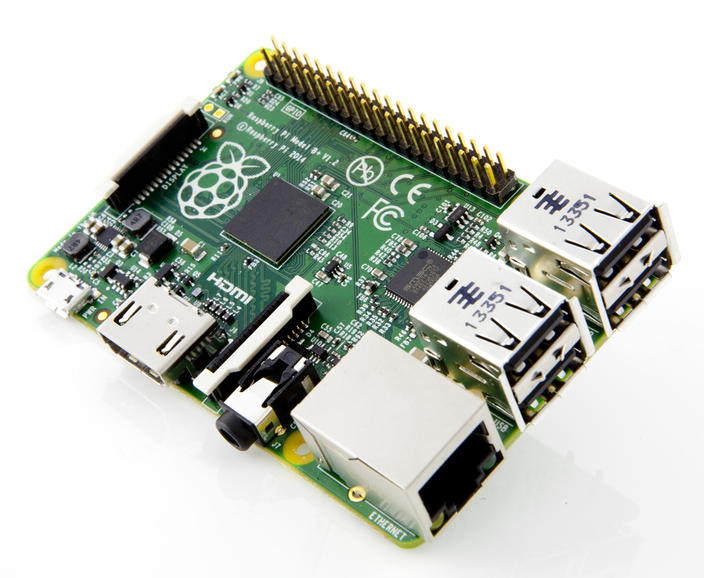
\includegraphics[scale=1]{../../fig/raspberry-pi-b-plus.jpg}
	\caption{Der Rasprberry Pi in der neusten Generation B+}
\end{figure}

Der Raspberry Pi ist als erste Wahl für die Rolle des Bordcomputers 
gewählt worden aufgrund der gegebenen Kriterien, zu denen folgende 
Ergebnisse zustande kamen.

\begin{description}
	\item[Fähigkeiten] Der Raspberry Pi ist in der Lage direkte
		LowLevel Ansteuerung durchzuführen mittels einer Vielzahl
		von Programmiersprachen. Dies ist insbesondere gegeben
		durch die Tatsache, dass ein vollwertiges Betriebsystem
		eingesetzt wird. Durch den Einsatz eines modernen
		Betriebssystems sind auch viele Erweiterungen für Hard- 
		und Software möglich, welche auch auf gewöhnlichen 
		Computern eingesetzt werden. Diese Eigenschaften erfüllen
		das Kriterium der disziplinären Zusammenführung in 
		optimaler Weise.
	\item[Einsatzbereitschaft] Der Raspberry Pi ist ein 
		Einplatinencomputer welcher (im Originalzustand vom 
		Hersteller) in wenigen Schritten in Betrieb genommen
		werden kann. 
	\item[Verbreitungsgrad] Der Raspberry Pi ist einer der
		populärsten Einplatinencomputer mit über 3 Millionen
		verfauften Exemplaren.
	\item[Leistung] Der Raspberry Pi ist nicht der Leistungssrärkste
		Vertreter unter den Einplatinencomputern, bietet dennoch
		gute Kennwerte und besitzt das beste
		Preis-Leistungsverhältnis mit dem geringen Preis.
	\item[Modifizierbarkeit] Der Raspberry Pi bietet ein vorbereitetes
		Interface an für eine Hardwareerweiterung, welches direkt
		die GPIO und Peripherie-IO zur Verfügung stellt. Auch
		für die Software ist eine hohe Modifizierbarkeit 
		gewährleistet durch den Einsatz von freien und 
		konfigurierbaren GNU/Linux Betriebssystemen.
	\item[Dokumentation] Da der Raspberry Pi explizit zu 
		Bildungs- und Experimentierzwechen entwickelt wurde, 
		bietet der Hersteller auch relevante Daten an für dessen
		Einsatz. Die Entwicklung im Bereich der
		erwerblichen Literatur oder der frei verfügbaren
		Tutorials korreliert mit den Verkaufszahlen und es 
		existieren grosse Benutzergemeindschaften.
	\item[Preis] Die Ziele der Raspberry Pi Foundation bei der
		Entwicklung des Raspberry Pi waren Kompaktheit und ein 
		niedriger Preis. Diese Ziele zeigen sich auch im
		entstandenen Produkt, welches bei offiziellen Distributor
		für 32.57 SFr. erworben werden kann. Dies ist ein 
		auffallend geringer Preis im Bereich der 
		Einplatinencomputer mit ähnlichen Eigenschaften.
\end{description}

Für die Evaluation ist ein aktuelles Modell eines Raspberry Pi mit
ArchLinux aufgesetzt worden. Dieses hat man überprüft auf die 
Lauffähigkeit gewisser Softwarekomponenten und Programmiersprachen,
was bisher positive Ergebnisse geliefert hat. Die bisherigen Ergebnisse
führten zudem zum Fazit, dass der Raspberry Pi ein für die Projektaufgabe
vielseitig einsetzbaren Bordcomputer darstellt, der hinsichtlich seiner
Einsatzfähigkeit nicht weiter untersucht werden muss.

Wie jede andere Komponente eines Systems, kann auch die des Bordcomputers
falsch eingeschätzt werden. Um ein späteres Nachsehen zu vermeiden wird
zu dieser Phase auch gleich evaluiert, wie man kritische Funktionen
aus- bzw. umlagern kann, falls der Raspberry Pi in dieses versagen sollte.

\subsubsection{LowLevel Fallback}
Sollte der Fall eintreten, dass gewisse LowLevel Funktionalitäten nicht
oder nur unter ungünstigen Bedingungen mit dem Raspberry Pi realisiert 
werden können, wird für diese Funktionen ein dediziertes LowLevel 
Mikrocontroller System hinzugezogen. Solche LowLevel Funktionen können
Hardware-Interrupts oder direkte Peripheriekomponenten des Mirkocontrollers
betreffen auf dem auch das Betriebssystem läuft. Diese LowLevel Funktionen
verlangen im Extremfall ein Anpassen des Kernels bzw. das erstellen eigener
Kernelmodule (Treiberprogramme). Der Overhead, welcher sich beim 
Kerneldevelopment ergeben kann, ist im Verhältnis zum Ergebnis suboptimal. 
Um auf solche Probleme ein Fallback zu haben wird ein einfaches 
Mikrocontrollersystem evaluiert welches ohne Betriebsystem auskommt und
dadurch wesentlich einfacher und dedizierter programmiert werden kann.

\begin{figure}[h!]
	\centering
	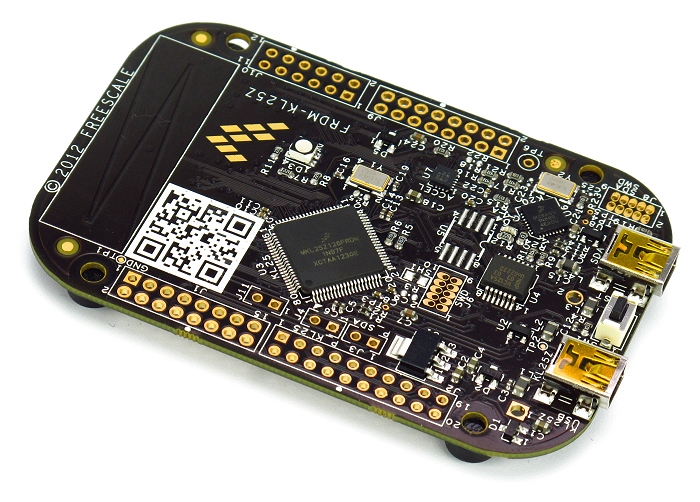
\includegraphics[scale=1]{../../fig/frdm-kl25z.jpg}
	\caption{Das Freedomboard FRDM-KL25Z von Freescale}
\end{figure}

Aktuell wird das Freedomboard FRDM-KL25Z evaluiert. Diese wird im Rahmen
des offiziellen Curriculum der Hochschule Luzern eingesetzt sowie auch
in einem aussercurricularem Kurs für Programmiereinsteiger. Die Vorteile,
welche sich dadurch ergeben sind erheblich, denn es besteht eine grosse
Benutzergruppe inklusive Dozenten auf dem Campus Horw welche Einführungen,
Kursunterlagen und sonstige Informationen und Hilfen anbieten können. Mit
Hilfe dieser Unterlagen war es bereits möglich die Buildutils der 
Hochschule auf Linux zu portieren. Mit einer Firmware des Herstellers und 
des OpenSDA ist es nun möglich ohne komplizierte Tools eigene Programme zu 
entwickeln und zu flashen ohne weitere Geräte. Im Falle eines plötzlichen 
Bedarfs für ein Fallback, sind dies entscheidende Kriterien. Zudem ergibt
sich wiederum die vorteilhafte Situation, dass auch die direkte 
Programmierung des Mikrocontrollers von den Informatik-Studenten erfolgen
kann und die geringe Manpower der Elektrotechnik entlastet werden kann
falls dies nötig ist.

\subsubsection{Alternativen}
